\documentclass[a4paper]{article}

\usepackage[top=1cm, bottom=1cm]{geometry}
\usepackage{graphicx}   % \graphicspath
\usepackage{setspace}   % {spacing}
\usepackage{color,soul} % \hl
\usepackage{relsize}    % \mathlarger
\usepackage{amsmath}    % \forall
\usepackage{amssymb}    % \mathbb
\usepackage{hyperref}   % \href
\usepackage{tikz}       % \tikz, \node
% \usepackage{showframe}


\hypersetup{colorlinks=true,urlcolor=cyan}

\renewcommand\labelitemi{\textperiodcentered}
% \textendash, \textperiodcentered

\graphicspath{{./assets/}}

\newcommand*\circled[1]{
        \tikz[baseline=(char.base)]{
                \node[shape=circle,draw,inner sep=1pt] (char) {#1};
        }
}


\begin{document}
        %%%%%%%%%%%%%%%%%%
        \section*{Vettori}
        %%%%%%%%%%%%%%%%%%

        \paragraph{Combinazione lineare:}
        Un vettore $y \in R^n$ si dice combinazione lineare dei vettori $v_1, ... , v_k$ se esistono $k$ moltiplicatori reali $w_1, ..., w_k$ tali che $v = \sum_{i=1}^{k} w_i v_i$.

        Ovvero, un vettore \`{e} combinazione lineare di altri vettori se il vettore \`{e} il risultato della somma degli altri vettori, ognuno di questi moltiplicato per una costante qualsiasi.

        \paragraph{Vettori linearmente indipendenti:}
        Un insieme di vettori \`{e} indipendente se \`{e} possibile ottenere il vettore nullo solamente con tutti i coefficienti $w_i$ uguali a $0$.

        Esempio: \quad $\{ (1, 0), (0, 1) \}$.

        \paragraph{Vettori linearmente dipendenti:}
        Un insieme di vettori \`{e} dipendente se \`{e} possibile ottenere il vettore nullo con almeno un coefficiente $w_i$ diverso da $0$.

        Un insieme che contiene il vettore nullo \`{e} linearmente dipendente.

        Esempio: \quad $\{ (1, 1), (2, 2) \}$.


        %%%%%%%%%%%%%%%%%%%%%%%%%%%%%%%
        \section*{Applicazioni lineari}
        %%%%%%%%%%%%%%%%%%%%%%%%%%%%%%%

        Una applicazione lineare o trasformazione lineare \`{e}:
        \begin{itemize}
                \item una funzione lineare tra due spazi vettoriali sullo stesso campo,
                \item ovvero una funzione che conserva le operazioni di somma di vettori e di moltiplicazione per uno scalare,
                \item ovvero una trasformazione lineare che preserva le combinazioni lineari,
                \item ovvero un omomorfismo di spazi vettoriali, in quanto conserva le operazioni che caratterizzano gli spazi vettoriali.
        \end{itemize}

        \paragraph{Condizione di linearit\`{a}:}
        $
                \forall \alpha, \beta \in \mathbb{K}
                \mbox{ e }
                \forall v_{1},v_{2} \in V
        $ \quad vale \quad
        $
                f(\alpha v_{1} + \beta v_{2}) = \alpha f(v_{1}) + \beta f(v_{2}).
        $

        \paragraph{Notazione matriciale:}
        Siano il vettore $v \in \mathbb{R}^n$ e $A = Mat(m, n, \mathbb{R})$, un'applicazione lineare $ f\!: \mathbb{R}^n \rightarrow \mathbb{R}^m $ si indica con $ f(v) = Av $.

        \paragraph{}
        $
                \begin{aligned}
                        f(v) & = f(x_1, \dots, x_n) \\
                             & = (a_{11} x_1 + \dots + a_{1n} x_n,\; \dots \;, a_{m1} x_1 + \dots + a_{mn} x_n) \\
                             & = Av =
                             \begin{bmatrix}
                                     a_{11}x_1 + \dots + a_{1n}x_n \\
                                     \vdots \\
                                     a_{m1}x_1 + \dots + a_{mn}x_n
                             \end{bmatrix} = \begin{bmatrix}
                                     a_{11} & \dots & a_{1n} \\
                                     \vdots & \ddots & \vdots \\
                                     a_{m1} & \dots & a_{mn}
                             \end{bmatrix} \begin{bmatrix}
                                     x_1 \\
                                     \vdots \\
                                     x_n
                             \end{bmatrix}.
                \end{aligned}
        $

        \paragraph{}
        Dalla definizione ne deriva che:
        \begin{itemize}
                \item il numero di righe \`{e} dato dal numero di variabili del dominio;
                \item il numero di colonne \`{e} dato dal numero di variabili del codominio.
        \end{itemize}

        \paragraph{Matrice canonica:}
        Con
        $
                f(e_1) = \begin{pmatrix} a_1 \\ b_1 \end{pmatrix},
                f(e_2) = \begin{pmatrix} a_2 \\ b_2 \end{pmatrix} \mbox{ ed }
                f(e_3) = \begin{pmatrix} a_3 \\ b_3 \end{pmatrix}
        $
        i vettori (linearmente indipendenti) della base canonica dell'applicazione lineare
        $
                f: \mathbb{R}^3 \rightarrow \mathbb{R}^2
        $,
        allora se
        $
                v = \begin{pmatrix} x \\ y \\ z \end{pmatrix}
        $
        \`{e} il vettore generico di $\mathbb{R}^3$:
        \[
                \begin{aligned}
                        f(v)    & = f \begin{pmatrix} x \\ y \\ z \end{pmatrix}
                                  = f(xe_1 + ye_2 + ze_3)
                                  = xf(e_1) + yf(e_2) + zf(e_3)
                                  = x \begin{pmatrix} a_1 \\ b_1 \end{pmatrix} + y \begin{pmatrix} a_2 \\ b_2 \end{pmatrix} + z \begin{pmatrix} a_3 \\ b_3 \end{pmatrix} \\
                                & = \begin{pmatrix}
                                        a_1 x + a_2 y  + a_3 z \\
                                        b_1 x + b_2 y + b_3 z
                                \end{pmatrix}
                                  = \begin{pmatrix}
                                        a_1 \mbox{ } a_2 \mbox{ } a_3 \\
                                        b_1 \mbox{ } b_2 \mbox{ } b_3
                                  \end{pmatrix}
                                  \begin{pmatrix} x \\ y \\ z \end{pmatrix}.
                \end{aligned}
        \]
        La matrice $A$ \`{e} detta matrice canonica di $f$, ed ha colonne
        $
                \begin{pmatrix}f(e_1) & \cdots & f(e_n)\end{pmatrix}
        $.

        \paragraph{Esempio:}
        Sia $f\;: \mathbb{R}^3 \to \mathbb{R}^3$ definita come segue:
        \[
                \begin{aligned}
                        f(0,1,1) & = (5,2,3); \\
                        f(2,0,0) & = (2,2,0); \\
                        f(1,1,0) & = (2,1,1); \\
                \end{aligned}
        \]

        La matrice rappresentativa dell'applicazione lineare va espressa tramite la base canonica,
        che quindi va ricavata.
        \[
                \begin{aligned}
                        f(1,0,0) & = f(2,0,0) / 2 = (2,2,0) / 2 = \underline{(1,1,0)}; \\
                        f(0,1,0) & = f(1,1,0) - f(1,0,0) = (2,1,1) - (1,1,0) = \underline{(1,0,1)}; \\
                        f(0,0,1) & = f(0,1,1) - f(0,1,0) = (5,2,3) - (1,0,1) = \underline{(4,2,2)}. \\
                \end{aligned}
        \]

        A questo punto la matrice rappresentativa \`{e} espressa con i vettori immagine in colonna.
        \[
                A = \begin{pmatrix}
                        1 & 1 & 4 \\
                        1 & 0 & 2 \\
                        0 & 1 & 2
                \end{pmatrix}.
        \]

        \paragraph{Esempio:}
        La matrice rappresentativa (rispetto alle basi canoniche) dell'applicazione lineare definita da
        $
                f(x,y,z) = (2x + 3y - z, 4x + 27y - 5z)
        $
        \`{e}
        \[
                A = \begin{pmatrix}
                        2 & 3  & -1 \\
                        4 & 27 & -5
                \end{pmatrix}.
        \]


        %%%%%%%%%%%%%%%%%%
        \section*{Matrici}
        %%%%%%%%%%%%%%%%%%
        \paragraph{Matrice triangolare superiore:}
        La riduzione di una \hl{matrice a scala} tramite il \hl{metodo di eliminazione di Gauss} genera una \hl{matrice triangolare superiore} con medesime soluzioni della matrice originale. \`{E}  utile per:
        \begin{itemize}
                \item risolvere sistemi lineari del tipo $ Ax = b $;
                \item determinare il \hl{rango} di una matrice (contando gli elementi di pivot non nulli).
        \end{itemize}

        \paragraph{Determinante:}
        Se il determinante di una matrice di vettori \`{e} diverso da $0$ allora i vettori sono \hl{linearmente indipendenti}.

        \paragraph{Rango di una matrice:}
        Si definisce rango di una matrice il massimo numero di vettori riga linearmente indipendenti tra loro o, equivalentemente, il massimo numero di vettori colonna linearmente indipendenti.

        \paragraph{Rango massimo:}
        Una matrice di $m$ righe per $n$ colonne pu\`{o} avere rango al massimo uguale a $min(m, n)$.
        Se il rango coincide con $min(m, n)$ allora \`{e} massimo.

        \paragraph{Matrice invertibile:}
        Una matrice \`{e} invertibile se e solo se ha \hl{rango massimo}, quindi determinante diverso da $0$.

        \paragraph{[HOWTO] Calcolo del rango:}
         \`{E} possibili determinare il rango di una matrice tramite:
        \begin{itemize}
                \item il \hl{criterio dei minori};
                \item il \hl{metodo di eliminazione di Gauss}.
        \end{itemize}

        \paragraph{Minori di ordine $j$:}
        Data una matrice di $m$ righe per $n$ colonne, un suo minore di ordine $j$ \`{e} una qualsiasi sottomatrice quadrata di ordine $j$, con $1 \leq j \leq min(m, n)$.

        \paragraph{[HOWTO] Criterio dei minori:}
        $j_i$ in prima istanza \`{e} $min(m, n)$.\\
        Se c'\`{e} almeno un minore di ordine $j_i$ con determinante diverso da $0$ allora il \hl{rango} della matrice originale \`{e} $j_i$.
        Se tutti i minori di ordine $j_i$ hanno determinante uguale a $0$ allora il rango della matrice \`{e} dato da $j_{i+1}$.
        L'$i$-esimo minore $j_i$, tranne il primo, ha ordine $j_{i-1} - 1$.

        \paragraph{[HOWTO] Eliminazione di Gauss:}
        $ R_{i} = R_{i} - \mathlarger{\frac{a_{i}}{a_{p}}} R_{p}$ dove $i$ \`{e} la riga corrente e $p$ \`{e} la riga di pivot.

        Se $a_{i}$ \`{e} $0$ si salta la riga essendo gi\`{a} a scalino e si procede con la successiva.

        Se l'elemento di pivot $a_{p}$ \`{e} $0$ si scambia la riga con un'altra il cui elemento di pivot \`{e} diverso da $0$.


        %%%%%%%%%%%%%%%%%%%%%%%%%%%%%%%%
        \section*{Sistema di generatori}
        %%%%%%%%%%%%%%%%%%%%%%%%%%%%%%%%
        Un sistema di generatori \`{e} un insieme di vettori che permette di ottenere tutti i vettori dello spazio mediante opportune combinazioni lineari.
        Con $V$ uno spazio vettoriale, $v, v_1, v_n$, vettori appartenenti a $V$ e $ a_1 \ldots a_n $ degli scalari appartenenti al campo $K$:

        $v = a_1 v_1 + a_2 v_2 + \ldots + a_n v_n = \mathlarger{\sum}_{i=1}^{n} a_i v_1$

        \paragraph{}
        Dato uno spazio vettoriale qualsiasi, non esiste un solo sistema di generatori.\\Per ogni spazio $V \neq {0}$ esistono infiniti sistemi di generatori.

        \paragraph{Basi e generatori:}
        \begin{itemize}
                \item Una base di uno spazio vettoriale \`{e} sempre un sistema di generatori;
                \item Un sistema di generatori non \`{e} necessariamente una base.
        \end{itemize}

        \paragraph{[HOWTO] Verifica di un sistema di generatori:}
        Un insieme di vettori \`{e} un sistema di generatori se la matrice (del sistema lineare associato all'insieme di vettori) ha \hl{rango massimo}.
        Se non ha rango massimo non \`{e} un sistema di generatori.

        \paragraph{Esempio:} ~\newline
        \begin{spacing}{1.7}
                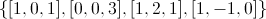
\includegraphics[scale=0.7]{55d6c70de6a2b6f5bfca5714bc322c0b}

                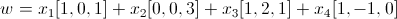
\includegraphics[scale=0.7]{b4b208240e420e9a59d7aee365987cea}

                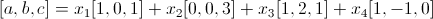
\includegraphics[scale=0.7]{c7f8c113a7a64f52390513751b40be1b}

                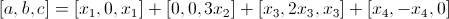
\includegraphics[scale=0.7]{8f6dcaecd7117937887835655f8e3955}

                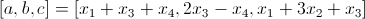
\includegraphics[scale=0.7]{34d0dd99a1b48b90aeb41fce06e193eb}

                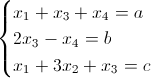
\includegraphics[scale=0.7]{624323dc4ef4c3a17e8e3b8e6fd97eda}

                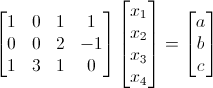
\includegraphics[scale=0.7]{7036093dfd160277402386a0104bb0b4}
        \end{spacing}

        Il rango \`{e} uguale a $3$, \`{e} massimo e quindi l'insieme di vettori \`{e} un sistema di generatori.


        %%%%%%%%%%%%%%%%%%%%%%%%%%%%
        \section*{Spazio vettoriale}
        %%%%%%%%%%%%%%%%%%%%%%%%%%%%
        \paragraph{Base di uno spazio vettoriale:}
        Un insieme di vettori $B$ \`{e} una base dello spazio vettoriale $V$ se $B$:
        \begin{itemize}
                \item \`{e} un sistema di generatori di $V$;
                \item \`{e} un sistema di vettori linearmente indipendenti.
        \end{itemize}

        \paragraph{Dimensione dello spazio:}
        La dimensione dello spazio vettoriale $V$, indicata con $dim(V)$, \`{e} il numero di elementi di una base qualsiasi di $V$.

        \href{http://www.youmath.it/domande-a-risposte/view/1318-quale-il-sottospazio-generato-da-questi-3-vettori-di-r3.html}{Sottospazio generato}

        \paragraph{Basi derivate da altre basi:}
        Disponendo di una base $B$ per lo spazio vettoriale $V$, tutte le basi che si ottengono moltiplicando i vettori di $B$ per scalari non nulli sono ancora basi di $V$ (distinte da $B$).

        \paragraph{Teorema dell'esistenza di una base:}
        Ogni spazio vettoriale ammette l'esistenza di una base.

        \paragraph{Teorema della non unicit\`{a} della base:}
        Ogni spazio vettoriale ammette infinite basi (se il campo di scalari \`{e} infinito).

        \paragraph{Cardinalit\`{a} delle basi:}
        Ogni base di uno spazio vettoriale $V$ ha la stessa cardinalit\`{a}, ovvero lo stesso numero di elementi.
        $\forall B,B'$ basi di $V \implies |B| = |B'|$

        \paragraph{}
        Da ci\`{o}, qualsiasi sistema di generatori avente un numero di vettori superiore alla dimensione dello spazio vettoriale non pu\`{o} costituire una base dello spazio stesso.

        \paragraph{Base di uno spazio vettoriale:}
        Una base di $\mathbb{R}^n$ \`{e} costituita esattamente da $n$ vettori.

        \paragraph{Base canonica di uno spazio vettoriale:}
        La base canonica di $\mathbb{R}^n$ \`{e} costituita esattamente da $n$ vettori ognuno dei quali ha una sola componente non nulla, ed ognuna di queste componenti non nulle \`{e} in una posione nel vettore diversa da tutti gli altri vettori.

        Esempio:
        Base canonica per $\mathbb{R}^3 = \{ \{1, 0, 0 \}, \{0, 1, 0\}, \{0, 0, 1\} \}$.

        \paragraph{[HOWTO] Estrarre una base da un sistema di generatori tramite il metodo di eliminazione di Gauss:}
        \begin{enumerate}
                \item si popola la matrice M con i vettori generatori (disposti per colonna);
                \item si riduce la matrice M tramite il metodo di eliminazione di Gauss ottenendo una mtrice M';
                \item le colonne di M' con pivot indicano in M (la matrice originale) le colonne che costituiscono una base.
        \end{enumerate}

        \paragraph{[HOWTO] Estrarre una base da un sistema di generatori tramite il criterio dei minori:}
        \begin{enumerate}
                \item si popola la matrice M con i vettori generatori (disposti per colonna);
                \item si usa il criterio dei minori per trovare una sottomatrice M' con $det(M') \neq 0$;
                \item le colonne di M' indicano in M (la matrice originale) le colonne che costituiscono una base; le colonne di M si prendono per intero anche se le righe di M' sono minori di M.
        \end{enumerate}


        %%%%%%%%%%%%%%%%%%%%%%%%%%%%%%%%%%%%
        \section*{Autovalore e autovettore:}
        %%%%%%%%%%%%%%%%%%%%%%%%%%%%%%%%%%%%
        Un numero complesso (o anche reale) $\lambda$ \`{e} un autovalore dell'endomorfismo $f: V \rightarrow V $, con $V$ uno spazio vettoriale su $\mathbb{R}$, $A_{f}$ la matrice associata-ad/rappresentativa-di $f$ rispetto ad una base di $V$ e $I$ la matrice identit\`{a} diagonale:
        \begin{itemize}
                \item se esiste un vettore $v \in V$ tale che $f(v) = \lambda v$;
                \item oppure se $A_{f}v = \lambda v$;
                \item oppure se $A_{f} - \lambda I$ non \`{e} invertibile, ovvero $det(A_{f} - \lambda I) = 0$.
        \end{itemize}

        Ovvero un vettore $v$ \`{e} un autovettore se differisce dalla sua immagine mediante $f$ solo per un multiplo scalare $c$.
        In questo contesto $v$ \`{e} un autovettore dell'autovalore $c$.

        Dire autovetorre ed autovalore della matrice $A_{f}$ significa autovettore ed autovalore dell'endomorfismo $f$ che ha $A_{f}$ come matrice associata/rappresentativa.

        \paragraph{[HOWTO] Trovare l'autovalore e l'autovettore:}
        Una matrice per non essere invertibile deve avere determinante uguale a $0$. Per cui:
        \[ det(A_{f} - \lambda I) = 0 \]
        In particolare il determinante della matrice $A_{f}$ \`{e} un polinomio in $\lambda$ detto polinomio caratteristico della matrice $A_{f}$. Gli autovalori della matrice sono gli zeri del polinomio caratteristico.

        \href{http://www.youmath.it/forum/algebra-lineare/66337-matrice-di-un-endomorfismo-con-il-vettore-immagine.html}{Matrice da vettori immagine}

        \href{http://www.youmath.it/forum/algebra-lineare/66469-matrice-associata-ad-un-endomorfismo-rispetto-a-due-basi-diverse.html}{Matrice rispetto a due basi}


        %%%%%%%%%%%%%%%%%%%
        \section*{Immagine}
        %%%%%%%%%%%%%%%%%%%
        Sia $F\!: D_{ominio} \to C_{odominio}$ un'applicazione lineare definita tra spazi vettoriali su un campo $\mathbb{K}$ (ad esempio $\mathbb{R}$), definiamo immagine di $F$:
        \[
                Im(F) = \{i \in C \;|\; \exists v \in D \mbox{ per cui } F(v) = i\}.
        \]

        \paragraph{[HOWTO] Come calcolare $dim(Im(F))$:}
        I vettori che costituiscono la matrice rappresentativa di un'applicazione lineare,
        indipendentemente dalla base a cui essi sono riferiti, costituiscono un sistema di generatori.

        \paragraph{}
        Per calcolare $dim(Im(F))$ si pu\`{o}:
        \begin{itemize}
                \item estrarre una base da un suo sistema di generatori e determinarne la dimensione;
                \item calcolare il rango di un suo sistema di generatori.
        \end{itemize}


        %%%%%%%%%%%%%%%%%%%%%%%%%%
        \section*{Nucleo o kernel}
        %%%%%%%%%%%%%%%%%%%%%%%%%%
        Sia $F\!: D_{ominio} \to C_{odominio}$ un'applicazione lineare definita tra spazi vettoriali su un campo $\mathbb{K}$ (ad esempio $\mathbb{R}$), definiamo il nucleo di $F$:
        \[
                Ker(F) = \{v \in D \;|\; F(v) = \underline{0} \in C\}
        \]

        Ovvero \`{e} l'insieme degli elementi del dominio che hanno immagine $\underline{0}$ mediante un'applicazione lineare definita su spazi vettoriali su un campo.

        \paragraph{Esempio:}
        Sia
        $ F\!: \mathbb{R}^{4} \to \mathbb{R}^{2} $
        definita da
        $
                A = \begin{pmatrix}
                        a_1 & b_1 & c_1 & d_1 \\
                        a_2 & b_2 & c_2 & d_2
                \end{pmatrix}
        $,
        allora
        $ Ker(F) \subset \mathbb{R}^{4} $
        ed \`{e} il sottoinsieme di vettori $x$ soluzione del sistema omogeneo $Ax = 0$.

        \paragraph{[HOWTO] Calcolo di $dim(Ker(F))$:}
        Sia $A$ la matrice associata all'applicazione lineare $F$, per calcolare $dim(Ker(F))$ \`{e} sufficiente trovare i vettori soluzione del sistema di equazioni $Ax = 0$.
        I vettori soluzione (anche solo uno) costituiscono una base del nucleo e la dimensione di questa base \`{e} la dimensione del nucleo.

        \paragraph{Dimensione:}
        Essendo il nucleo un sottospazio del dominio, ne deriva che $0 \leq dim(Ker(F)) \leq dim(D)$.
        \begin{itemize}
                \item Se $dim(Ker(F)) = 0$, allora l'unico elemento del nucleo \`{e} \underline{0}.
                \item Se $dim(Ker(F))) = dim(D)$, allora $Ker(F) = D$ ed $F$ \`{e} l'applicazione lineare che associa ad ogni elemento di $D$ lo zero di $C$.
        \end{itemize}

        \paragraph{Teorema dell'iniettivit\`{a}:}
        $F$ \`{e} iniettiva se e solo se $Ker(F) = \{ \underline{0} \}$, ovvero se e solo se $F$ ha nucleo banale.

        \paragraph{Teorema di nullit\`{a} pi\`{u} rango (o teorema del rango o teorema della dimensione):}
        \[
                dim(D) = dim(Ker(F)) + dim(Im(F))
        \]


        %%%%%%%%%%%%%%%%%%%%%%%%%%%%%%
        \section*{Equazioni diofantee}
        %%%%%%%%%%%%%%%%%%%%%%%%%%%%%%
        \paragraph{Minimo comune multiplo (mcm):}
        $
                \mathlarger{\frac{a \times b}{MCD(a, b)}}.
        $

        \paragraph{Massimo comune divisore (MCD) (algoritmo di Euclide):} ~\newline

        $a = qb + r$.

        $MCD(N, n)$:
        {
                \setlength{\tabcolsep}{1pt}
                \begin{tabular}{r l l l}
                        N = & n & * $q_1$ + $r_1$ \\
                        n = & $r_1$  & * $q_2$ + $r_2$ \\
                        $r_1$  = & $r_2$  & * $q_3$ + $r_3$ \\
                        \ldots = & \ldots & * \ldots + \ldots \\
                        $r_h$  = & $r_{h+1}$   & * $q_{h+2}$ + \circled{$r_{h+2}$} \\
                        $r_{h+1}$ = & $r_{h+2}$   & * $r_{h+1}$ + \ul{0}
                \end{tabular} $ \quad \implies \quad r_{h+2}$.
        }

        \paragraph{Teorema di B\'{e}zout:}
        Se $a,b$ sono interi e $(a,b)$ \`{e} il loro massimo comune divisore,
        allora esistono interi $h,k$ tali che
        \[ ha + kb = (a, b). \]

        \paragraph{Esempio:}
        $132 h + 51 k = 3$

        \paragraph{}
        \makebox[\width]{
                $MCD(132, 51)$:
                {
                        \setlength{\tabcolsep}{1pt}
                        \begin{tabular}{r l l l}
                                132 = & 51 & * 2 + 30 ; \\
                                 51 = & 30 & * 1 + 21 ; \\
                                 30 = & 21 & * 1 + 9 ; \\
                                 21 = & 9 & * 2 + \circled{3} ; \\
                                  9 = & 3 & * 3 + \ul{0} ;
                        \end{tabular}
                }
        } $\implies$
        \makebox[\width]{
                $
                        \begin{aligned}
                                \underline{3}
                                & = 21 - 2 \cdot 9 \\
                                & = 21 - 2 (30 - 21) \\
                                & = -2 \cdot 30 + 3 \cdot 21 \\
                                & = -2 \cdot 30 + 3 (51 - 30) \\
                                & = 3 \cdot 51 - 5 \cdot 30 \\
                                & = 3 \cdot 51 - 5 (132 - 2 \cdot 51) \\
                                & = \underline{13 \cdot 51 - 5 \cdot 132}.
                        \end{aligned}
                $
        }


        %%%%%%%%%%%%%%%%%%%%%%%
        \section*{Permutazioni}
        %%%%%%%%%%%%%%%%%%%%%%%
        Con $S_n$ si intende l'insieme di permutazioni composte dai numeri che vannno da $1$ a $n$.

        Se in una permutazione non compare un numero, questo vuol dire che va in se stesso.


        %%%%%%%%%%%%%%%%%%%%%%%%%%%
        \section*{Numeri complessi}
        %%%%%%%%%%%%%%%%%%%%%%%%%%%
        \paragraph{Forma cartesiana}:
        \[ z = x + iy \mbox{\quad dove \quad} Re(z) = x,\ Im(z) = y. \]


        \paragraph{Forma esponenziale:}
        $ z = |z| \ (\mbox{cos}\theta + i \ \mbox{sin}\theta)$

        Dove \quad $x = Re(z) = |z|cos\theta$ \quad e \quad $y = Im(z) = |z|sin\theta$.

        \paragraph{Modulo:}
        $ r = |z| = \sqrt{x^2 + y^2} $.

        \paragraph{Argomento:}
        $
                \theta = Arg(z) \in (-\pi,+\pi] =
                \begin{cases}
                        \arccos{\left( \mathlarger{\frac{x}{|z|}} \right) \mbox{ se } y \geq 0} \\
                        -\arccos{\left( \mathlarger{\frac{x}{|z|}} \right) \mbox{ se } y < 0} \\
                \end{cases} =
                \begin{cases}
                        \frac{\pi}{2} \mbox{ se } x = 0, \ y > 0 \\
                        -\frac{\pi}{2} \mbox{ se } x = 0, \ y < 0 \\
                        \mbox{non definito se } x = 0, \ y = 0 \\
                        \arctan{\left(\frac{y}{x}\right)} \mbox{ se } x > 0, \ y \mbox{ qualsiasi} \\
                        \arctan{\left(\frac{y}{x}\right)} + \pi \mbox{ se } x < 0, \ y \geq 0 \\
                        \arctan{\left(\frac{y}{x}\right)} - \pi \mbox{ se } x < 0, \ y < 0
                \end{cases}
        $

        $
                \theta = Arg(z) \in [0,2\pi) = \begin{cases}
                        \frac{\pi}{2} \mbox{ se } x = 0, \ y > 0 \\
                        \frac{3\pi}{2} \mbox{ se } x = 0, \ y < 0 \\
                        \mbox{non definito se } x = 0, \ y = 0 \\
                        \arctan{\left(\frac{y}{x}\right)} \mbox{ se } x > 0 , y \ge 0 \\
                        \arctan{\left(\frac{y}{x}\right)} + 2 \pi \mbox{ se } x > 0, y < 0 \\
                        \mbox{TODO: manca una condizione}
                \end{cases}
        $

        \paragraph{}
        \href{http://www.youmath.it/lezioni/analisi-matematica/numeri-complessi/760-calcolare-le-radici-di-un-numero-complesso.html}{Calcolo delle radici di un numero complesso}


        \newpage
        %%%%%%%%%%%%%%%%%
        \section*{Gruppi}
        %%%%%%%%%%%%%%%%%
        Un gruppo $(G, \ast)$ \`{e} una coppia composta da un insieme $G$ ed un'operazione $\ast$ su $G$ che:
        \begin{itemize}
                \item risulti essere associativa, ovvero $(a \ast b) \ast c = a \ast (b \ast c)$;
                \item ammetta un elemento neutro $i$, ovvero $g \ast i = i \ast g = g \quad \forall g \in G$;
                \item rispetto alla quale ogni elemento di $G$ risulti invertibile, ovvero $a \ast a_{inv} = i$.
        \end{itemize}

        \paragraph{}
        Un gruppo la cui operazione \`{e} commutativa \`{e} detto \hl{gruppo abeliano}.

        \paragraph{}
        Un sottogruppo di un gruppo deve godere delle stesse propriet\`{a} del gruppo, pi\`{u}:
        \[ \forall a,b \in S \subseteq G \quad a \ast b \in S\]


        %%%%%%%%%%%%%%%%%
        \section*{Anelli}
        %%%%%%%%%%%%%%%%%
        Un insieme $(A, +, \times)$ dotato di due operazioni, dette somma e prodotto, \`{e} detto anello se:
        \begin{itemize}
                \item $(A,+)$ \`{e} un gruppo abeliano con elemento neutro $0_A$;
                \item $\times$ \`{e} associativa con elemento neutro $1_A$;
                \item vale la legge distributiva del prodotto rispetto alla somma: $\forall a,b,c \in A \quad a \times (b + c) = a \times b + a \times c \mbox{ e } (b + c) \times a = b \times a + c \times a$;
                \item $0_A \not= 1_A$.
        \end{itemize}


        %%%%%%%%%%%%%%%%
        \section*{Campi}
        %%%%%%%%%%%%%%%%
        Un insieme $(C, +, \times)$ dotato di due operazioni, dette somma e prodotto, \`{e} detto campo se:
        \begin{itemize}
                \item $(C,+)$ \`{e} un gruppo abeliano con elemento neutro $0_C$;
                \item $(C,\times) \backslash \{0_C\}$ \`{e} un gruppo abeliano con elemento neutro $1_C$;
                \item vale la legge distributiva del prodotto rispetto alla somma: $\forall a,b,c \in C \quad a(b+c) = ab+ac \mbox{ e } (b+c)a = ba+ca$.
        \end{itemize}


        %%%%%%%%%%%%%%%%%%%%%%
        \section*{Omomorfismi}
        %%%%%%%%%%%%%%%%%%%%%%
        Dati due gruppi G e G', \newline
        un \textbf{omomorfismo} \`{e} una funzione $f\!: G \to G'$ tale che
        \[
                f(ab) = f(a)f(b).
        \]

        \paragraph{}
        Dati due gruppi $(G, +)$ e $(G', \times)$, \newline
        un \textbf{omomorfismo di gruppi} \`{e} una funzione $f\!: G \to G'$ tale che $\forall a,b \in G$
        \[
                f(a + b) = f(a) \times f(b).
        \]

        \paragraph{}
        Dati due anelli $(A, +, \times)$ e $(A', +', \times')$, \newline
        un \textbf{omomorfismo di anelli} \`{e} una funzione $f\!: A \to A'\,\! $ tale che $\forall a,b \in A$
        \[
                \begin{aligned}
                        f(a + b)     & = f(a) +' f(b), \\
                        f(a \times b) & = f(a) \times' f(b).
                \end{aligned}
        \]

        Se l’operazione di prodotto definita in $A$ gode della propriet\`{a} commutativa diremo che $A$ \`{e} un anello commutativo.

        \paragraph{Isomorfismi:}
        Un isomorfismo \`{e} un omomorfismo biettivo.

        Un esempio sono le matrici triangolari superiori.

        \paragraph{Teorema fondamentale dell'isomorfismo:}
        Dati due gruppi $ G, G^{\prime} $, un sottogruppo normale $N$ di $G$ ed un omomorfismo $ f:\ G \to G^{\prime} $
        con nucleo $ Ker(f) = N $, esiste un unico isomorfismo $ \overline{f}:\ G/N \to f(g) \mid f = \overline{f}(\pi(x)) $. In particolare l'immagine di $f$ \`{e} un gruppo isomorfo a $ G / N$.

        \paragraph{Immagine:}
        \`{E} l'immagine $\in G'$ dell'applicazione lineare su $G$.

        \paragraph{Nucleo:}
        \`{E} l'insieme degli elementi $\in G$ che tramite l'applicazione lineare vengono trasformati nell'identit\`{a} di $G'$.


        %%%%%%%%%%%%%%%%%%%%%
        \section*{Partizioni}
        %%%%%%%%%%%%%%%%%%%%%
        Una partizione di un insieme \`{e} una suddivisione dell'insieme in sottoinsieme disgiunti.


        %%%%%%%%%%%%%%%%%%%%%%%%%%%%%%%%%%%
        \section*{Relazioni di equivalenza}
        %%%%%%%%%%%%%%%%%%%%%%%%%%%%%%%%%%%
        Una relazione di equivalenza \`{e} una relazione che soddisfa le seguenti propriet\`{a}:
        \begin{description}
                \item[(transitiva)] se $a \sim b$ e $b \sim c$, allora $a \sim c$;
                \item[(simmetrica)] se $a \sim b$ allora $b \sim a$;
                \item[(riflessiva)] $a \sim a \quad \forall a \in S$.
        \end{description}

        \paragraph{Classi di equivalenza:}
        Un sottoinsieme di $A$ che contiene tutti e soli gli elementi equivalenti a un qualche elemento $x \in A$ prende il nome di classe di equivalenza di $x$ per la relazione $\sim$ e si indica con $[x]_\sim$.
        In una classe di equivalenza tutti gli elementi in essa contenuti sono tra loro equivalenti.

        \paragraph{}
        Sia $G$ un gruppo e $H$ un suo sottogruppo normale ($gH = Hg$), $[g] = Hg = gH = [g]^{*}$.


        %%%%%%%%%%%%%%%%%%%%%%%%%%
        \section*{Classi laterali}
        %%%%%%%%%%%%%%%%%%%%%%%%%%
        \paragraph{Laterale destro:}
        $Hx = \{ hx \mid h \in H \mbox{ e } x \in Hx \}$

        \paragraph{Laterale sinitro:}
        $xH = \{ xh \mid h \in H \mbox{ e } x \in xH \}$

        \paragraph{}
        Se H \`{e} un insieme finito si ha che $|H| = |Hx| = |xH| \quad \forall x \in G$.

        \paragraph{Teorema di Lagrange:}
        Se $G$ \`{e} un gruppo finito ed $H$ un suo sottogruppo allora $|G| = r|H|$ dove r \`{e} il numero dei laterali destri o sinistri di $H$ in $G$.
        Ovvero l'ordine di $H$ divide l'ordine di $G$.

        \paragraph{}
        Le classi laterali sono classi di equivalenza rispetto alla relazione di congruenza:
        \[ a \equiv b, \mbox{ se } b = ah \mbox{ per qualche } h \in H \]
        e costituiscono una partizione del gruppo.


        %%%%%%%%%%%%%%%%%%%%%%%%%%%
        \section*{Gruppi quoziente}
        %%%%%%%%%%%%%%%%%%%%%%%%%%%
        L'insieme delle classi di equivalenza su $A$ si chiama insieme quoziente di $A$ per la relazione $\sim$, e viene indicato con l'espressione $A / \sim$.

        Sia $G$ un gruppo ed $H$ un sottogruppo di $G$, $ G / H = \{ [g] \mid g \in G \}$.


        %%%%%%%%%%%%%%%%%%%%%
        \section*{Congruenze}
        %%%%%%%%%%%%%%%%%%%%%
        Dato un intero positivo $n$, due numeri interi $a, b$ sono congrui modulo $n$, indicati con $a \equiv b \mbox{ mod } n$, se $a - b$ \`{e} divisibile per $n$, ovvero se esiste un numero intero $h$ tale che $a - b = hn$.

        \paragraph{Propriet\`{a} elementari:}
        \begin{enumerate}
                \item se $a \equiv a' \mbox{ mod } n$ e $b \equiv b' \mbox{ mod } n$ allora $a + b \equiv a' + b' \mbox{ mod } n$; equivalentemente se $[a]_n = [a']_n$ e $[a]_n = [a']_n$ allora $[a + b]_n = [a' + b']_n$;
                \item se $a \equiv a' \mbox{ mod } n$ e $b \equiv b' \mbox{ mod } n$ allora $ab \equiv a'b' \mbox{ mod } n$; equivalentemente se $[a]_n = [a']_n$ e $[a]_n = [a']_n$ allora $[ab]_n = [a'b']_n$;
                \item $a \equiv 0 \mbox{ mod } n$ se e solo se $n$ divide a se e solo se $[a]_n =[0]_n$;
                \item $r$ \`{e} il resto della divisione di $a$ per $n$ se e solo se $0 \leq r < n$ e $[a]_n = [r]_n$;
                \item $(a+b) \mbox{ mod } n = (( a \mbox{ mod } n) + (b \mbox{ mod } n)) \mbox{ mod } n$.
                \item $(ab) \mbox{ mod } n= ((a \mbox{ mod } n) \cdot (b \mbox{ mod } n)) \mbox{ mod } n$.
        \end{enumerate}

        \paragraph{Congruenze lineari:}
        Guarda gli Appunti di Norberto Gavioli, da pagina 4.

        \paragraph{}
        Sia $ax \equiv b \mbox{ mod } n$, allora una soluzione esiste solo se $(a,n)$ divide b.

        Si ha $ax - b = hn$  e quindi $b = ax - hn$ \`{e} un multiplo di $(a,n)$.

        Se $x$ \`{e} una soluzione allora \`{e} una soluzione anche $x + \mathlarger{\frac{zn}{(a,n)}}$ $\forall z \in \mathbb{Z}$.


        %%%%%%%%%%%%%%%%%%%%%%%%%%
        \section*{Classi di resto}
        %%%%%%%%%%%%%%%%%%%%%%%%%%
        \paragraph{Lemma:}
        Siano $a$ ed $n$ due numeri interi primi tra loro e si supponga che $n$ divida il prodotto $ab$ dove $b \in \mathbb{Z}$; allora $n$ divide $b$.

        Ci sono esattamente $n$ classi di resto modulo $n$: $[0]_n, [1]_n, \ldots, [n - 1]_n$.

        \paragraph{}
        Parlando delle classi di resto modulo $n$, la classe di resto $[r]_n$ di un intero $r$ \`{e} data da tutti gli interi che si ottengono da $r$ aggiungendo un multiplo di $n$: $[r]_n = \{ r + kn \;|\; k \in \mathbb{Z}\} = r + n \mathbb{Z}$.

        \noindent
        Ovvero una classe di resto $r$ modulo $n$ \`{e} un insieme  di numeri interi relativi che divisi per $n$ danno lo stesso resto $r$.

        \noindent
        Ovvero una classe di resto modulo $n$ non \`{e} altro che un laterale del sottogruppo $n \mathbb{Z}$ di $\mathbb{Z}$.

        \paragraph{}
        Le classi di resto modulo $n$ sono esattamente $n$.


        %%%%%%%%%%%%%%%%%%%%%%%%%%%%%%%%%%%%%%%
        \section*{Dim. del Teorema di Lagrange}
        %%%%%%%%%%%%%%%%%%%%%%%%%%%%%%%%%%%%%%%
        Poich\'{e} $\sim$ \`{e} una relazione di equivalenza, i laterali destri $Hg$ formano esattamente $ G:H $
        sottoinsiemi disgiunti essendo partizioni, ciascuno dei quali contiene esattamente $|H|$ elementi, poich\'{e}
        $ |H| = |Hx| = |xH|$.  Ne segue che $ |G| = |G:H| \cdot |H| $.

\end{document}
